\subsection{Testbed Commissioning and Telemetry Validation}
\label{subsec:testbed-commissioning}

Prior to the execution of the full $N=30$ trial batteries across the experimental groups, the testbed underwent systematic commissioning and functional validation. This stage verified that the deployment manifests, container runtimes, telemetry pipelines, and fault-injection hooks interact as specified in the architectural design.

\begin{figure}[htbp]
  \centering
  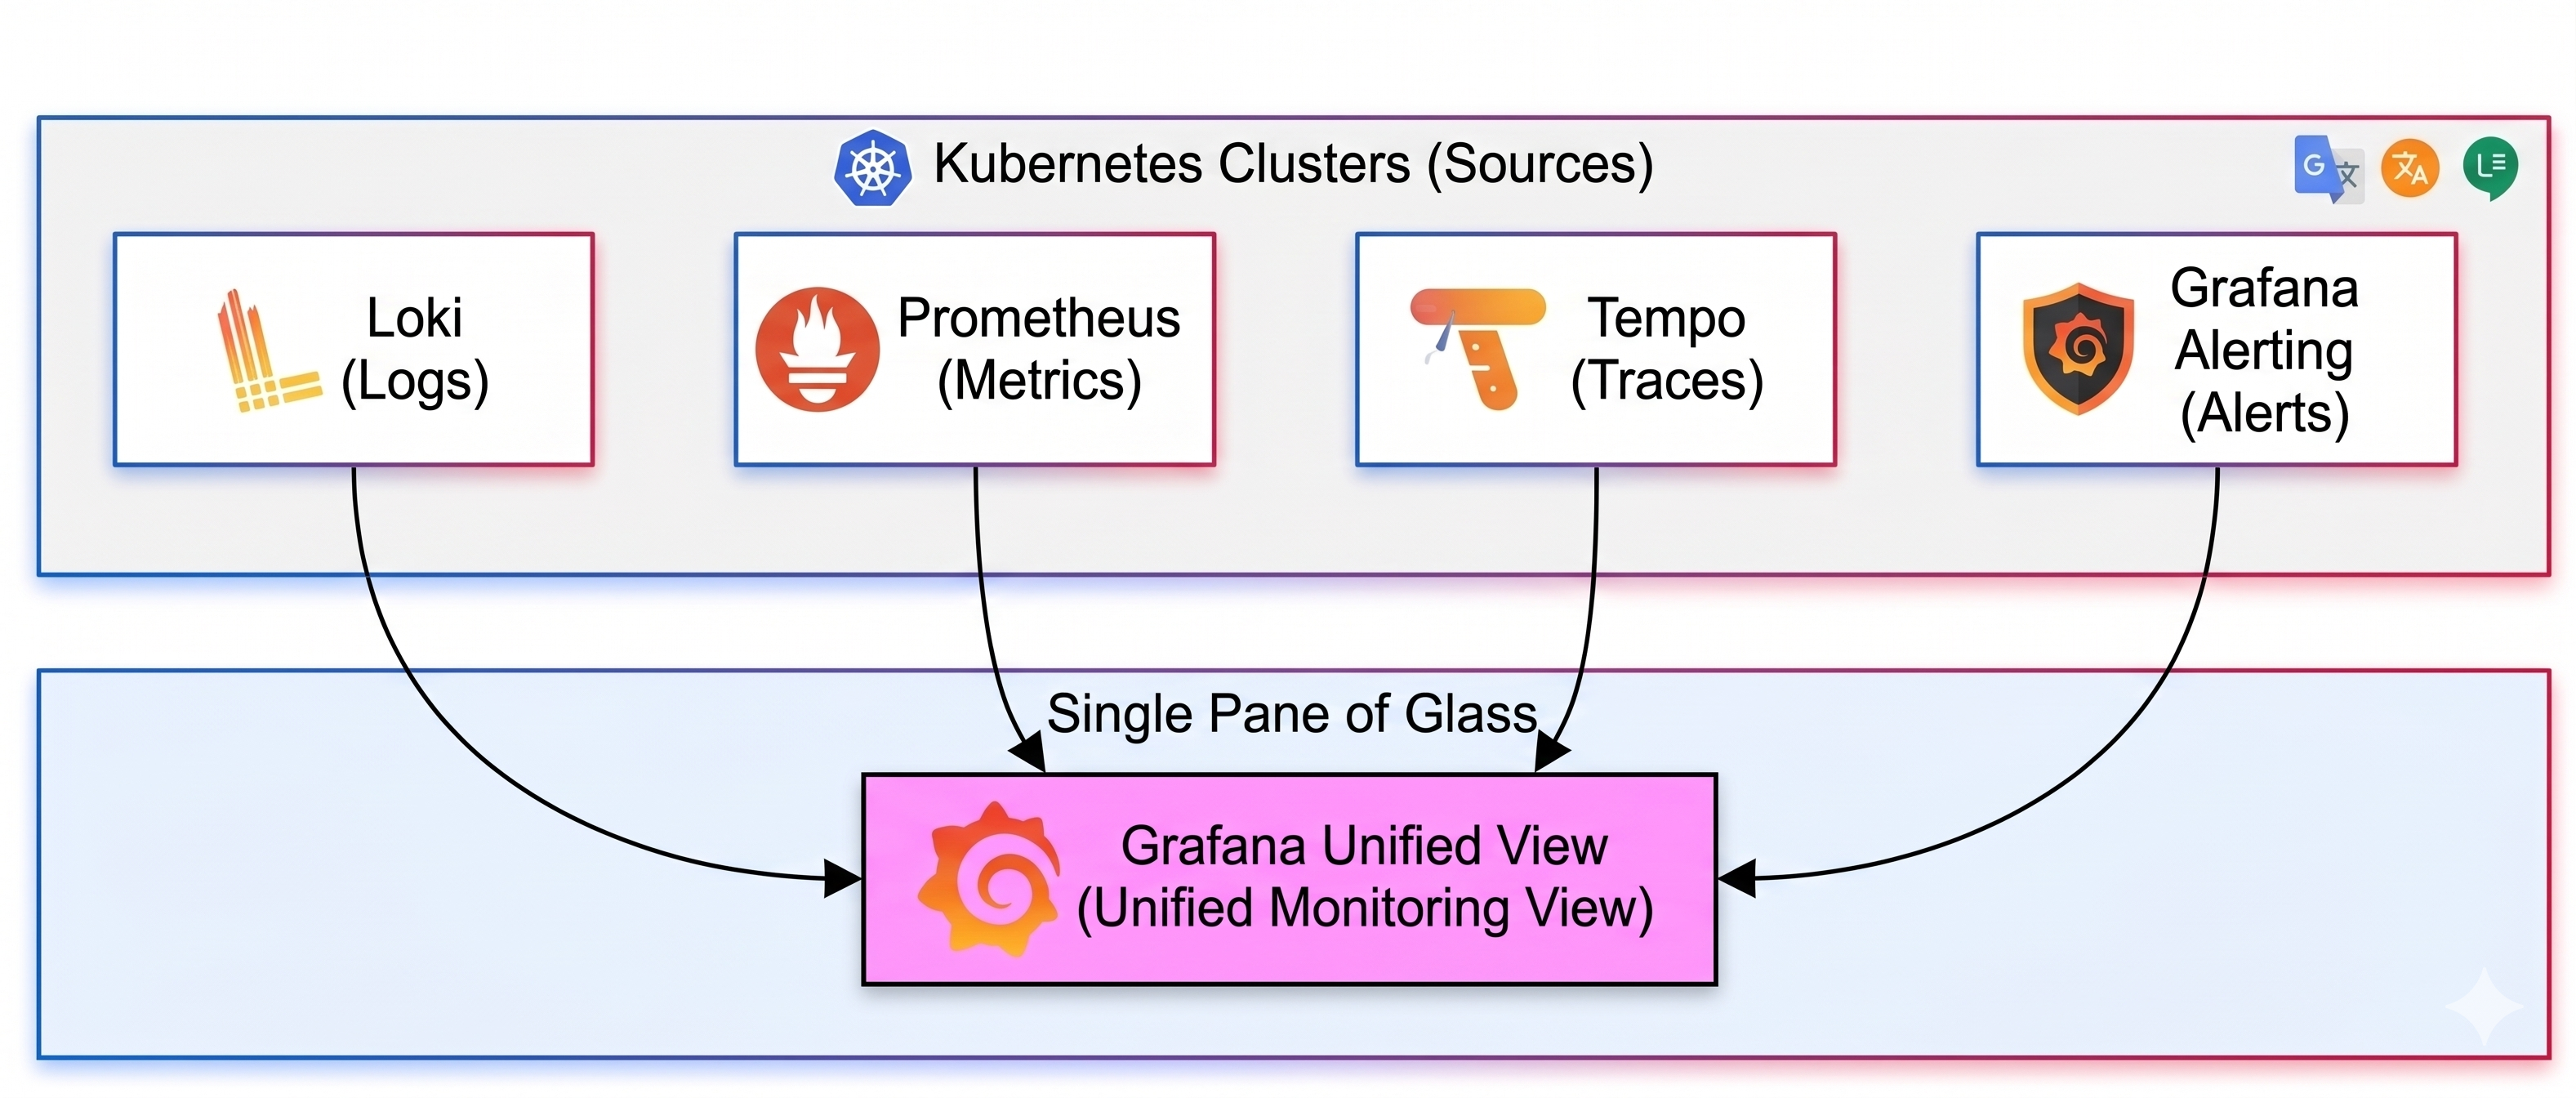
\includegraphics[width=0.9\textwidth]{images/experiment/grafana_preliminary.png}
  \caption{Single Pane of Glass dashboard validating unified telemetry ingestion in Grafana.}
  \label{fig:grafana_preliminary}
\end{figure}

Figure~\ref{fig:grafana_preliminary} demonstrates the operational ``Single Pane of Glass'' dashboard during steady-state workload execution. It validates that the OpenTelemetry collectors actively extract spans, runtime metrics, and container logs from the polyglot microservices, successfully streaming them to their respective storage backends: Prometheus, Grafana Loki, and Grafana Tempo. Furthermore, controlled perturbation trials confirmed that Chaos Mesh successfully manipulates the network namespaces of the target pods (applying netem delays) without destabilizing the underlying K3s control plane, establishing the safety and repeatability of the fault injection mechanism.

While the empirical evaluation of diagnostic latency ($MTTDiag$) is conducted autonomously via programmatic APIs to eliminate human operator bias, Grafana serves as the operational supervisory layer. It validates the underlying semantic binding implemented across the datasource configurations:
\begin{itemize}
    \item \textbf{Metrics to Traces via Exemplars:} The Prometheus datasource binds OpenTelemetry \texttt{traceID} values to latency histograms as exemplars. When an anomalous duration is recorded in the upper latency percentiles ($p95/p99$), the associated exemplar exposes the exact \texttt{traceID}, enabling immediate transition to the corresponding trace graph in Grafana Tempo without manual cross-system lookup.
    
    \item \textbf{Traces to Logs via Contextual Bindings:} The Tempo datasource integrates an automated \textit{Trace to Logs} mapping. For any anomalous span identified within a degraded execution path, the engine synthesizes a LogQL query for Loki. By scoping the search to the specific span timeframe, container namespace, and \texttt{traceID}, it bridges the gap between detecting inter-service latency inflation and inspecting the underlying execution context.
\end{itemize}

These integrated correlation pathways provide interactive root cause navigation within the Grafana interface for post-mortem analysis, while the deterministic RCA engine in Scenario~4 navigates this exact semantic topology programmatically via HTTP endpoints.